\vspace{-.5ex}
\section{Further Examples}\label{sec:examples}
\vspace{-.5ex}

\vspace{-.5ex}
\subsection{Concurrent Spanning Tree}\label{subsec:CSTExample}
\vspace{-.5ex}

Programs manipulating arbitrary graphs present the following significant
challenge for compositional verification: because of deep sharing
between different components of a graph, changes to one subgraph may
affect other subgraphs which may point into it. This makes it hard to
reason about updates to each subgraph in isolation. In a concurrent
setting, this difficulty compounds with the fact that threads working
on different parts of the graph may affect each other in ways that are
difficult to reason about locally to each subgraph. Central to those
issues is the fact that different subgraphs present \emph{unspecified
  sharing} and may overlap in arbitrary ways. We now demonstrate on a
concurrent spanning tree example that \colosl may be just the tool you
need in this case, as it naturally deals with arbitrary overlapping
views of the shared state, and allows one to tailor interferences to a
given subjective view.

Our example, presented in \fig\ref{fig:conSpanningTree}, operates on a
\emph{directed binary graph} (henceforth simply \emph{graph}),
\textit{i.e.} a directed graph where each node has at most two
successors, called its left and right children. The program computes a
in-place spanning tree of the graph, \textit{i.e.} a tree that covers
all nodes of the graphs from a given root, concurrently as follows:
each time a new node is encountered, two new threads are created that
each prune the edges of the left and right children recursively. A
mark bit is associated to each node to keep track of which ones have
already been visited. Each thread returns whether the root
of the subgraph it was operating on had already been visited; if so,
the parent thread removes the link from its root node to the
corresponding child. Intuitively, it is allowed to do so because,
since the child was marked by another thread, the child has to be
already reachable via some other path in the graph.

%% marking the vertices to keep track of those already visited; the
%% return value b records the outcome of marking with \li{b}$=1$ when the
%% top node $x$ is unmarked (not visited yet) and \li{b}$=0$
%% otherwise. Assuming that the root vertex $x$ is unmarked initially,
%% the algorithm continues by first marking $x$ and subsequently spanning
%% the left and right subgraphs concurrently. When the top node of the
%% left subgraph is already marked (\li{!b1}), the edge from $x$ into it
%% is replaced by a null pointer. This corresponds to the case where the
%% node has already been visited by another thread and is thus reachable
%% from the root; \emph{mutatis mutandis} for the right subgraph.

We will prove that, given a shared graph as input, the program always
returns a tree, \textit{i.e.} all sharing and cycles have been
appropriately removed. Pleasingly, the \colosl specification achieves
maximal locality and allows us to reason only on the current subgraph
manipulated by a thread, instead of the whole graph. Because of
arbitrary sharing between the two, a global specification would be
unpleasant indeed!  However, we do not establish that the final tree
indeed spans the original graph. The reason it does is subtle indeed,
as are the invariants required, but in ways unrelated to our main
issue, which is to provide tight specifications for each thread.

To reason about this program, following Hobor and
Villard~\cite{ramification}, we use two representations of graphs. The
first is a mathematical representation $\gamma = (V, E)$ where $V$ is
a finite set of vertices and $E: V \rightarrow (V \uplus
\{\li{null}\}) \times (V \uplus \{\li{null}\})$ is a function
associating each vertex with at most two successors, where \li{null}
denotes the absence of an edge from the node.  We write $n \in \gamma$
for $n \in V$, $\gamma(n)$ for $E(n)$ and $|\gamma|$ for $|V|$.


%% Jules: definition of spanning tree is wrong (what's minimal?) since
%% graphs need not be connected now. Not needed anyway, as we don't
%% show that we have a spanning tree.
%% 
%% Similarly, let $\theta = (V, E)$ denote an \emph{acyclic} DCB graph
%% with no sharing between subgraphs, \textit{i.e.}, a \emph{tree}. For
%% brevity, in this section we refer to a DCB graph and an acyclic DCB
%% graph simply as a graph and a tree, respectively. Given a graph
%% $\gamma$, a tree $\theta$ \emph{spans} $\gamma$ if it includes all
%% vertices of $\gamma$ with a minimal set of edges where every edge in
%% $\theta$ is also an edge in $\gamma$.  For instance,
%% \fig\ref{fig:graphAndTree} depicts a DCB graph and a possible spanning
%% tree where the dashed lines indicate those edges that have been
%% removed from the graph after spanning it.



\begin{wrapfigure}[8]{r}{0.3\columnwidth}
	\centering
	\begin{tabular}{|c |}
		\hline
			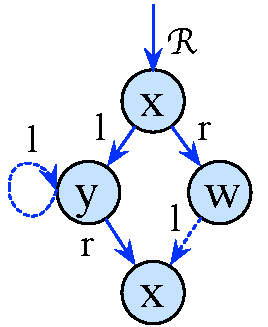
\includegraphics[scale=0.27]{Sections/FurtherExamples/Images/graph.pdf} \\
		\hline
	\end{tabular}
\caption{A graph.}
\label{fig:graphAndTree}
\end{wrapfigure}
%%
%\begin{figure}
%\hrule
%\begin{tabular}{c c c}
%	\begin{subfigure}[b]{0.3\columnwidth}
%      \centering	
%      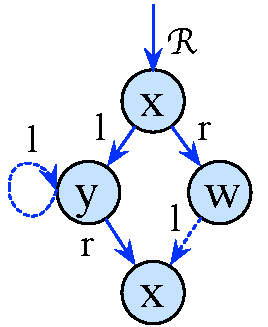
\includegraphics[scale=0.3]{Sections/FurtherExamples/Images/graph.pdf}
%    \caption{}
%    \label{subfig:graph}
%    \end{subfigure}
%    &
%    \begin{subfigure}[b]	{0.2\columnwidth}		
%      \centering	
%      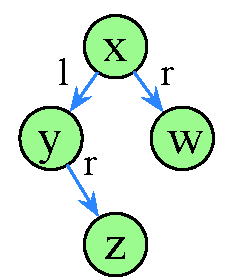
\includegraphics[scale=0.3]{Sections/FurtherExamples/Images/tree.pdf}
%    \caption{}
%    \label{subfig:tree}
%    \end{subfigure}
%    &
%    \begin{subfigure}[b]{0.3\columnwidth}
%      \centering	
%      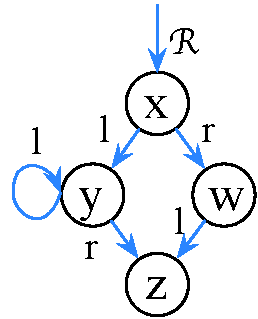
\includegraphics[scale=0.3]{Sections/FurtherExamples/Images/graphWithRootEdge.pdf}
%    \caption{}
%    \label{subfig:graphWithRootEdge}
%    \end{subfigure}
%    \end{tabular}
%\hrule
%\caption{A directed connected binary graph (\subref{subfig:graph}), a possible spanning tree (\subref{subfig:tree}), and the same graph with the logical edge $\rootEdge$ (\subref{subfig:graphWithRootEdge}).}
%\label{fig:graphAndTree}
%\end{figure}
%%

Mathematical graphs are connected to a second, in-memory
representation by an inductive predicate $\graph{x}{\gamma}$, denoting
a spatial (in-heap) graph rooted at address $x$ corresponding to the
mathematical graph $\gamma$. The predicate definition uses the
overlapping conjunction to account for the sharing between the left
and right children and for potential cycles in the graph, as shown in
\fig\ref{fig:globalCST}.  The basic action we allow on spatial graphs
is to \emph{mark} a node, changing its mark field from $0$ to $1$ and
claiming ownership of its left and right pointers in the process. Such
an action is allowed by a \emph{marking} capability of the form
$\markT{n}{e}$ where $n$ denotes the vertex (address) and $e$ the edge
via which vertex $n$ is visited. For instance, the capabilities
associated with marking of vertex $z$ in \fig\ref{fig:graphAndTree}
are $\markT{z}{y.r}$ and $\markT{z}{w.l}$. Note that the
parameterisation of our actions are merely a notational convenience
and can be substituted for their full definitions. Given a graph at
root address $x$, in order to account for the ability to mark the root
vertex $x$, we introduce a logical (virtual) root edge $\rootEdge$
into $x$ as depicted in \fig\ref{fig:graphAndTree} together with its
associated marking capability $\markT{x}{\rootEdge}$. The shared state
contains node $x$ which can be either unmarked ($\unmarked{x}{l}{r}$)
or marked ($\marked{x}$); as well as the left and right subgraphs
captured recursively by $\G{l}{\gamma}$ and $\G{r}{\gamma}$.
%% Note that the two subgraphs and vertex $x$ are combined by
%% the overlapping conjunction $\sepish$ since the graph can be cyclic
%% and each node may be reachable via more than one path.

Each vertex is represented as three consecutive cells in the heap
tracking the mark bit and the addresses of the left ($l$) and right
($r$) subgraphs. For brevity, we write $\cell{x}{m, l, r}$ for
$\cell{x}{m} * \cell{x+1}{l} * \cell{x+2}{r}$, and $x.m$, $x.l$, and
$x.r$ for $x$, $x+1$, and $x+2$, respectively. When vertex $x$ is in
the unmarked state, the whole cell $\cell{x}{0,l,r}$ and the
capabilities to mark the children reside in the shared state. In the
marked state, the shared state only contains $\cell{x.m}{1}$: the left
and right subgraphs (pointers and capabilities) have been claimed by
the thread who marked the node, while other threads need not access
the children of $x$ once they see that $x$ is already marked. The
atomic \li{CAS} instruction prevents several threads to concurrently
mark the same node and claim ownership of the same resource.

The interference associated with the graph is described as the union
of interferences pertaining to the vertices of the graph ($n \in
\gamma$). For each vertex $n \in \gamma$, the only permitted action is
that of marking $n$ which can be carried out by any of the marking
capabilities associated with node $n$ ($\markT{n}{-}$). Note that the
anonymous quantification $-$ is yet another notational shorthand and
can be substituted for the following more verbose definition.
%
\vspace{-1ex}
\[
\vspace{-1ex}
I(n) \eqdef \bigcup\limits_{p \in \gamma} \left(\bigcup_{e \in \{p.l,
  p.r, \rootEdge\}}\!\!\! \markT{n}{e} : \exsts{l, r} \unmarked{n}{l}{r} \swap \marked{n} \right)
\]
%
%
\begin{figure}
%
\hrule
\[
\begin{array}{r @{\hspace*{2pt}} l}
	\graph{x}{\gamma} \eqdef & \left[\markT{x}{\rootEdge}\right] * \shared{\G{x}{\gamma}}{I_\gamma} \hspace*{0.5cm} I_\gamma \eqdef \bigcup\limits_{n \in \gamma}I(n)\\
%	
	\G{x}{\gamma} \eqdef & (x = \li{null} \land \emp) \lor x \in \gamma \land \exsts{l, r} \gamma(x) = (l, r) \\
	& \land \left( \unmarked{x}{l}{r} \lor \marked{x}\right) \sepish \G{l}{\gamma} \sepish \G{r}{\gamma}\\
%
	\unmarked{x}{l}{r} \eqdef & \cell{x}{0, l, r} * \left[\markT{l}{x.l}\right] * \left[\markT{r}{x.r} \right]\\
%	
	\marked{x} \eqdef & \cell{x}{1}\\
%
	I(n) \eqdef & \left\{ \markT{n}{-}: \exsts{l, r} \unmarked{n}{l}{r} \swap \marked{n}\right\}\\
%
%	\tree{x}{\gamma} \eqdef & \markT{x}{\rootEdge} * \shared{\G{x}{\gamma}}{\bigcup\limits_{n \in \gamma}I(n)}\\
\end{array}
\]
%
\hrule
\vspace{-6pt}
\caption{Global specification of the graph predicate.}
\label{fig:globalCST}
\end{figure}
%
%
\fig\ref{fig:conSpanningTree} shows an in place concurrent algorithm for calculating a spanning tree of a graph. It proceeds by 
%
\begin{figure}
%
\hrule
\[
\begin{array}{r @{\hspace*{2pt}} l}
	\g{x}{\gamma} \eqdef & (x = \li{null} \land \emp) \lor x \in \gamma \land \exsts{l, r} \gamma(x) = (l, r) \land\\
	& \shared{\unmarked{x}{l}{r} \lor \marked{x}}{I(x)} * \g{l}{\gamma} * \g{r}{\gamma}\\
	
	\tr{x}{\gamma} \eqdef & (x = \li{null} \land \emp) \lor x \in \gamma \land \exsts{l, r} \gamma(x) = (l, r) \land\\
	& \shared{\marked{x}}{I(x)} *  \exsts{l' \in \{l, \li{null}\}} \exsts{r' \in \{r, \li{null}\}}\\
	& \left[\markT{l}{x.l}\right] * \cell{x.l}{l'} * \tr{l'}{\gamma} * \\
	& \left[\markT{r}{x.r}\right] * \cell{x.r}{r'} * \tr{r'}{\gamma}
\end{array}
\]
\hrule
\vspace{-6pt}
\caption{Local specification of the graph predicate.}
\label{fig:localCST}
\end{figure}
%
The $\graph{x}{\gamma}$ predicate defined in \fig\ref{fig:globalCST} is a \emph{global} account of the graph in that it captures all vertices and the interference associated with them. However, our spanning tree algorithm operates \emph{locally} as it is called upon recursively for each node. That is, for each \li{span(n)} call (where $\cell{\li{n}}{n}$ and $n \in \gamma$), the footprint of the call is limited to node $n$. Moreover, in order to reason about the concurrent recursive calls $\li{span(x.l)} || \li{span(x.r)}$, we need to \emph{split} the state into two $*$-composed states prior to the calls, pass each constituent state onto the relevant thread and combine the resulting states by $*$ composition through an application of the \parRule\ rule. We thus provide a \emph{local} specification of the graph, $\g{x}{\gamma}$ as defined in \fig\ref{fig:localCST} such that for all $n, p \in \gamma$ and $e \in \{p.l, p.r, \rootEdge \}$
%
\vspace{-1ex}
\[
\begin{array}{@{} c @{} }
	\color{blue}{
	\Big\{
		\cell{\li{n}}{n} * \cell{\li{b}}{-} * 
		\left[\markT{n}{e}\right] * 
		\g{n}{\gamma}
	\Big\} 
	} \\
%	
	\command{b:= span(n)} \\ 
%
	\color{blue}{
	\Big\{
		\cell{\li{n}}{n} *  
		\left[\markT{n}{e}\right] * 
		\left(
%		\begin{array}{@{} l @{}}
			\cell{\li{b}}{1} * \tr{n}{\gamma} \lor
			\cell{\li{b}}{0} *  \tr{\li{null}}{\gamma}
%		\end{array}
		\right)
	\Big\}
	}
\end{array}
\]
%
The definition of the $\g{x}{\gamma}$ predicate is similar to that of $\shared{\G{x}{\gamma}}{I_{\gamma}}$ except that the global view $\shared{\G{x}{\gamma}}{I_{\gamma}}$ that describes the resources associated with all $|\gamma|$ vertices has been replaced by $|\gamma|$ $*$-composed more local views, each describing the resources of a vertex $n \in \gamma$. Moreover, the interference of each local view concerning a vertex $n \in \gamma$ has been shifted from $I_{\gamma}$ to $I(n)$ as to reflect only those actions that affect $n$.  

Similarly, the $\tr{x}{\gamma}$ predicate represents a \emph{tree}
rooted at $x$, as is standard in separation logic~\cite{rey02}, and
consists of $|\gamma|$ subjective views one for each vertex in
$\gamma$. The assertion of each subjective view reflects that the
corresponding vertex ($x$) has been marked
$\shared{\marked{x}}{I(x)}$. The resources associated with each node
$x$, namely the left and right pointers and the corresponding marking
capabilities have been claimed by the marking thread and moved into
the local state. The vertex addressed by the left pointer of $x$
(\textit{i.e.} $l'$) corresponds to either the initial value prior to
marking ($l$ where $\gamma(x) = (l, r)$) or \li{null}\ when $l$ has
more than one predecessors and has been marked by another thread,
making the whole predicate stable against actions of the program and
the environment.

We now demonstrate how to obtain the local specification $\g{x}{\gamma}$ from the global specification of \fig\ref{fig:globalCST}. 
When expanding the definition of $\G{x}{\gamma}$, there are two cases to consider depending on whether or not $x = \li{null}$. In what follows we only consider the case where $x \not= \li{null}$ since the derivation in the case of $x = \li{null}$ is trivial.
Let
%
\vspace{-1ex}
\[
\begin{array}{l l}
	P \eqdef & \iterStar_{n \in \gamma} \left( \gamma(n) = (l, r) \land (\unmarked{n}{l}{r} \lor \marked{n}) \; \right)\\
	
	Q \eqdef & \iterStar_{n \in \gamma} \left( \gamma(n) = (l, r) \land \shared{\unmarked{n}{l}{r} \lor \marked{n}}{I(n)} \right)\\
\end{array}	
\]
%
Then we have $\G{x}{\gamma} \iff  P$ and $\g{x}{\gamma} \iff Q$.
%% %
%% \[
%% \begin{array}{l @{\hspace*{1cm}} c @{\hspace*{1cm}} l}
%% 	\G{x}{\gamma} \iff  P & \text{and} & \g{x}{\gamma} \iff Q
%% \end{array}
%% \]
%% %
It thus suffices to show $\shared{P}{I_{\gamma}} \semimplies Q$.
%
\begin{align*}
	\shared{P}{I_{\gamma}} &
	\stackrel{(\textsc{Copy})}{\implies}
	\underbrace{\shared{P}{I_{\gamma}} * \cdots * \shared{P}{I_{\gamma}}}_{|\gamma| \text{ times}}\\
	&\stackrel{(\textsc{Forget})}{\implies}
	\iterStar_{n \in \gamma} \left( \gamma(n) = (l, r) \land \shared{\unmarked{n}{l}{r} \lor \marked{n}}{I_{\gamma}}  \right)\\
	& \stackrel{(\textsc{Shift})}{\semimplies}
	\iterStar_{n \in \gamma} \left( \gamma(n) = (l, r) \land \shared{\unmarked{n}{l}{r} \lor \marked{n}}{I(n)}  \right)\\
	&\iffdef Q
\end{align*}
%
%%
%\[
%\begin{array}{@{} c @{} l @{}}
%	&\shared{P}{\bigcup\limits_{n \in S} I(n)}  \\
%	
%	\stackrel{(\textsf{G}\ \defin)}{\implies} & \shared{\exsts{l, r} (\unmarked{x}{l}{r} \lor \marked{x}) \sepish \G{l}{S} \sepish \G{r}{S}}{\bigcup\limits_{n \in S} I(n)} \\
%	
%	\implies &   \exsts{l, r}  \shared{(\unmarked{x}{l}{r} \lor \marked{x}) \sepish \G{l}{S} \sepish \G{r}{S}}{\bigcup\limits_{n \in S} I(n)} \\
%	
%	\stackrel{(\textsc{Copy})}{\implies} &
%	\exsts{l, r}  
%	\shared{(\unmarked{x}{l}{r} \lor \marked{x})  \sepish \G{l}{S} \sepish \G{r}{S}}{\bigcup\limits_{n \in S} I(n)} \\
%	& * \shared{(\unmarked{x}{l}{r} \lor \marked{x}) \sepish \G{l}{S} \sepish \G{r}{S}}{\bigcup\limits_{n \in S} I(n)} \\
%	& * \shared{(\unmarked{x}{l}{r} \lor \marked{x})  \sepish \G{l}{S} \sepish \G{r}{S}}{\bigcup\limits_{n \in S} I(n)} \\
%	
%	
%	\stackrel{(\textsc{Forget})}{\implies} &
%	\exsts{l, r}  
%	\shared{\unmarked{x}{l}{r} \lor \marked{x}  }{\bigcup\limits_{n \in S} I(n)} \\
%	& * \shared{\G{l}{S}}{\bigcup\limits_{n \in S} I(n)} * \shared{\G{r}{S}}{\bigcup\limits_{n \in S} I(n)} \\
%	
%	
%	
%	\stackrel{(?)}{\semimplies} &
%	\exsts{l, r}  
%	\shared{\unmarked{x}{l}{r} \lor \marked{x}}{\bigcup\limits_{n \in S} I(n)} * \g{l}{S} * \g{r}{S}\\
%	
%	
%	\stackrel{(\textsc{Shift})}{\semimplies} &
%	\exsts{l, r}  
%	\shared{\unmarked{x}{l}{r} \lor \marked{x} }{I(x)} * \g{l}{S} * \g{r}{S}\\
%	
%	
%	\iffdef & \g{x}{S}
%	
%\end{array}
%\]
%%
%
\begin{figure}
\hrule
\begin{lstlisting}
 //$\comment\{ \cell{\tx{x}}{x} * \cell{\tx{b}}{-} * \graph{x}{\gamma}\}$
 //$\comment\{\cell{\tx{x}}{x} *  \cell{\tx{b}}{-} * \markT{x}{\rootEdge} * \shared{\G{x}{\gamma}}{I_{\gamma}}\}$
 //$\comment\{\cell{\tx{x}}{x} * \cell{\tx{b}}{-} * \left[\markT{x}{\rootEdge}\right] * \g{x}{\gamma}\}$
 b:= span(x) $\{$
   //$\comment\left\{\begin{array}{l} \cell{\tx{x}}{x} * \cell{\tx{b}}{-} * \left[\markT{x}{\rootEdge}\right]\\ * \exsts{l, r} \shared{\unmarked{x}{l}{r} \lor \marked{x}}{I(x)} * \g{l}{\gamma} * \g{r}{\gamma} \end{array} \right\}$
   res:= $\langle$ CAS(x.m, 0, 1) $\rangle$;
   //$\comment\left\{\begin{array}{l} \cell{\tx{x}}{x} * \cell{\tx{b}}{-} * \left[\markT{x}{\rootEdge}\right] * \shared{\marked{x}}{I(x)} *\\ \exsts{l, r} \g{l}{\gamma} * \g{r}{\gamma} *\\ \left(\cell{\tx{res}}{0} \lor  \left(\begin{array}{l} \cell{\tx{res}}{1} * \cell{x.l}{l} * \cell{x.r}{r}\\ * \left[\markT{l}{x.l}\right] * \left[\markT{r}{x.r}\right] \end{array}\right)\right)\end{array}\right\}$
   if (res) then $\{$ 
   //$\comment\left\{\begin{array}{l} \cell{\tx{x}}{x} * \cell{\tx{b}}{-} * \left[\markT{x}{\rootEdge} \right] * \shared{\marked{x}}{I(x)} \\\cell{\tx{res}}{1} * \exsts{l, r} * \cell{x.l}{l} * \cell{x.r}{r} *\\ \left[\markT{l}{x.l} \right] * \g{l}{\gamma} * \left[\markT{r}{x.r}\right] * \g{r}{\gamma}  \end{array} \right\}$
     //$\comment\left\{ \left[\markT{l}{x.l} \right] * \g{l}{\gamma} * \left[\markT{r}{x.r} \right] * \g{r}{\gamma}  \right\}$   
     b1:= span(x.l) || b2:= span(x.r)
     //$\comment\left\{\begin{array}{@{} l @{}}  \left[\markT{l}{x.l} \right] * \left( (\cell{\tx{b1}}{1} *  \tr{l}{\gamma}) \lor \cell{\tx{b1}}{0}\right) *\\ \left[ \markT{r}{x.r} \right] * \left( (\cell{\tx{b2}}{1} * \tr{r}{\gamma}) \lor \cell{\tx{b2}}{0} \right)  \end{array}\right\}$   
   //$\comment\left\{\begin{array}{@{} l @{} }  \cell{\tx{x}}{x} * \cell{\tx{b}}{-} * \left[ \markT{x}{\rootEdge} \right] * \shared{\marked{x}}{I(x)} \\\cell{\tx{res}}{1} * \exsts{l, r} * \cell{x.l}{l} * \cell{x}{r} *\\ \left[ \markT{l}{x.l} \right] * \left( (\cell{\tx{b1}}{1} *  \tr{l}{\gamma}) \lor \cell{\tx{b1}}{0} \right) *\\ \left[ \markT{r}{x.r} \right] * \left( (\cell{\tx{b2}}{1} * \tr{r}{\gamma}) \lor \cell{\tx{b2}}{0} \right)    \end{array}\right\}$  
     if (!b1) then 
       $\text{[}$x.l$\text{]}$:= null
     if (!b2) then 
       $\text{[}$x.r$\text{]}$:= null
   //$\comment\left\{\begin{array}{l}  \cell{\tx{x}}{x} * \cell{\tx{b}}{-} * \left[ \markT{x}{\rootEdge} \right] * \shared{\marked{x}}{I(x)} * \\ \cell{\tx{res}}{1} * \cell{\tx{b1}}{-} * \cell{\tx{b2}}{-} *  \exsts{l, r}  \\ \exsts{l' \in \{l, \tx{null}\}} \left[ \markT{l}{x.l} \right] * \cell{x.l}{l'} * \tr{l'}{\gamma} *\\ \exsts{r' \in \{r, \tx{null}\}} \left[ \markT{r}{x.r} \right] * \cell{x.r}{r'} * \tr{r'}{\gamma} \end{array}\right\}$  
   //$\comment\left\{\begin{array}{l}  \cell{\tx{x}}{x} * \cell{\tx{b}}{-} * \cell{\tx{res}}{1} *\cell{\tx{b1}}{-} * \cell{\tx{b2}}{-}\\ * \markT{x}{\rootEdge} *  \tr{x}{\gamma}  \\  \end{array}\right\}$         
   $\}$ //$\comment\left\{ \begin{array}{l @{}} \cell{\tx{x}}{x} * \cell{\tx{b}}{-} * \left[ \markT{x}{\rootEdge} \right]*  \\  (\cell{\tx{res}}{1}  * \tr{x}{\gamma}) \lor \left(\begin{array}{@{} l @{}}\cell{\tx{res}}{0} * \shared{\marked{x}}{I(x)} \\  * \g{l}{\gamma} * \g{r}{\gamma} \end{array}\right) \end{array} \right\}$ 
   //$\comment\left\{ \begin{array}{l} \cell{\tx{x}}{x} * \cell{\tx{b}}{-} * \left[ \markT{x}{\rootEdge} \right] *  \\  (\cell{\tx{res}}{1}  * \tr{x}{\gamma}) \lor (\cell{\tx{res}}{0} ) \end{array} \right\}$      
   return res
 $\}$ //$\comment\left\{ \begin{array}{@{} l @{}} \cell{\tx{x}}{x}  * \left[ \markT{x}{\rootEdge} \right] *  ((\cell{\tx{b}}{1}  * \tr{x}{\gamma}) \lor \cell{\tx{b}}{0}) \end{array} \right\}$         
\end{lstlisting}
\hrule\vspace*{-6pt}
\caption{Concurrent Spanning Tree Implementation}
\label{fig:conSpanningTree}
\end{figure}
%
%
\vspace{-2ex}
\subsection{Set Module}
\vspace{-.5ex}
\label{sec:set}
In this section we consider a concurrent set module and explore a pictorial specification. We first revisit the set specification of Concurrent Abstract Predicates (CAP) in~\cite{cap-ecoop10}; we then compare it against our specification in \colosl. We demonstrate that our \colosl\ reasoning considerably improves on CAP by producing a \emph{more concise} specification and allowing for \emph{more local} reasoning. 

We implement a set as a sorted singly-linked list with no duplicate elements (since it represents a set) and one lock per node as described in~\cite{cap-ecoop10}. Our set module provides three functionalities: \li{contains(v)}, \li{add(v)} and \li{remove(v)}.
%The $\inSet{\var{h}}{\var{v}} $ predicate asserts that the set at \var{h} contains value \var{v}. Dually, $\outSet{\var{h}}{\var{v}}$ asserts that the set does not contain \var{v}. 
As the name suggests, the \li{contains(v)} function checks whether value \var{v} is contained in the set; the \li{add(v)} and \command{remove(v)} functions add/remove value \var{v} to/from the list, respectively.
%
All three operations proceed by traversing the sorted list from the head address and locating the first node in the list holding a value $v'$ greater than or equal to $v$. The algorithm for locating such a node begins by locking the head node; it then moves down the list by hand-over-hand locking whereby first the node following the one currently held is locked and subsequently the previously locked node is released. 
%

The following diagram illustrates the set predicate in CAP.\\
%
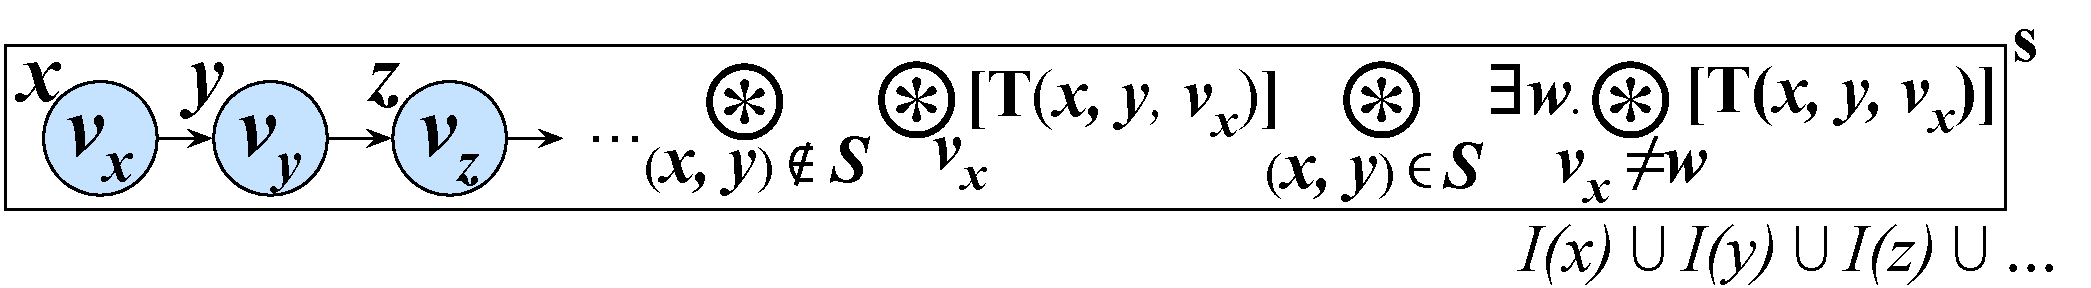
\includegraphics[scale=0.232]{Sections/FurtherExamples/Images/capSet.pdf}\\
%
%In this specification all elements of the set (represented as a singly-linked list) reside in a shared region labelled $s$ and the interference on the set is the combined interference associated with each node in the list. Since the capabilities associated with a region can only be allocated upon region creation, the shared region is required to keep track of all possible update capabilities $[\text{U}(x, y, v_{x})]$ associated with all addresses $x$, all possible successor addresses $y$ and all values $v_{x}$. For instance, since the value $v_{x}$ may be contained in the set at address $x$ before address $y$, the region must include the $[\text{U}(x, y, v_{x})]$ capability to accommodate possible modifications of value $v_{x}$. This is captured by the infinite multiplicative star operator $\iterStar$. It uses an auxiliary mathematical set $S$ to track those nodes of the list that are currently locked and thus infer which \text{U} capabilities reside in the shared state and which ones have been removed. This results in an inevitably cluttered and a rather counter-intuitive specification since it seems unnatural to account for the capabilities pertaining to addresses not in the domain of the set. 
%
%
In this specification, the elements of the list are represented as a singly-linked list where the list starts at address $x$ with value $v_1$ and points to the next element at address $y$ with value $v_2$ and so forth. In the remainder of this section, we write $\node{x}{v}{y}$ to denote a node at address $x$, with value $v$ and successor $y$. 

All nodes of the list reside in a single shared region labelled $s$ and the interference on the list is the combined interference associated with each constituent node. 
Each node at a given address $x$, is associated with a set of update capabilities of the form $[\text{U}(x, y, v)]$ for \emph{all} possible addresses $y$ and \emph{all} possible values $v$. This is to capture all potential successor addresses $y$ and all potential values $v$ that may be stored at address $x$. For instance, since the value $v_{1}$ may be contained in the list at address $x$ before address $y$, there must exist an update capability $[\text{U}(x, y, v_1)]$ to accommodate possible modifications of value $v_{1}$ with respect to $x$ and $y$. In order to modify a node, a thread can acquire the lock associated with the node and subsequently claim the relevant update capability.
% 

Since in CAP the capabilities associated with a region can only be generated upon region creation, the shared region is required to keep track of all possible update capabilities $[\text{U}(x, y, v)]$ associated with all addresses $x$ (including those not currently in the domain of the list), all addresses $y$ and all values $v$. At any one point, given $\node{x}{v}{y}$, the only update capability that can be claimed by a thread (through locking) is the one that reflects its current status, namely $[\text{U}(x, y, v)]$. As a result, an auxiliary mathematical set $S$ is used to track those nodes of the list that are currently locked and thus infer which $[\text{U}]$ capabilities have been claimed. The distribution of update capabilities is captured by the two assertions written as the \emph{infinite multiplicative star operator} $\iterStar$. The first part of the assertion states that given any node at address $x$ with successor $y$, if it is not locked, \textit{i.e.} $(x, y) \not\in S$, then \emph{all} of its update capabilities of the form $[\text{U}(x, y, v)]$ lie in the shared region for \emph{all} values $v$. On the other hand, if it is locked, \textit{i.e.} $(x, y) \in S$, then the update capabilities for \emph{all} values $v$ \emph{but one} ($w \not= v$) are in the shared region.

This specification is unnecessarily complicated. It is rather counter-intuitive to account for the capabilities pertaining to addresses not in the domain of the list. Moreover, it is overly verbose to consider all combinations of values and successor addresses. Lastly, each thread is required to ``know'' of the resources associated with all nodes in the list and account for their associated interference. 

%
We proceed with the \colosl\ specification of the set module. Recall from \S\ref{sec:logic} that \colosl\ is parametric in the separation algebra of capabilities. We thus instantiate it with a heap-like capability separation algebra that is \emph{stateful} and demonstrate that this allows for a more concise specification.  

We specify the set predicate as the *-composition of the subjective views pertaining to each node in the singly-linked list as illustrated below. The interference on each subjective view is limited to the node in question. Associated with each node at address $x$, is a ``next'' capability $\nextC{x}{y}$ that tracks its successor $y$. This capability is analogous to the $[\text{U}(x, y, v)]$ capability of CAP and we shortly demonstrate how it is utilised in our reasoning.

%
{\centering 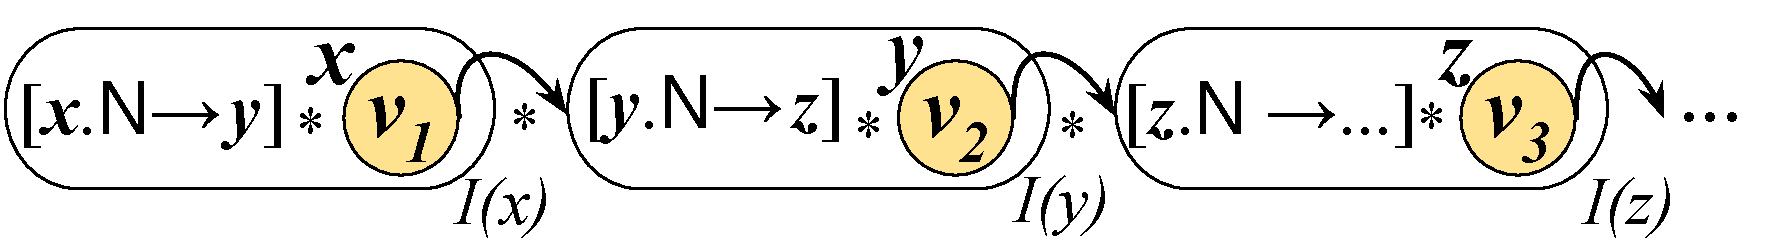
\includegraphics[scale=0.24]{Sections/FurtherExamples/Images/coloslSet.pdf}\\}
%
\noindent Since \colosl\ allows for \emph{dynamic} extension of the shared state, we do not need to account for capabilities associated with \emph{all} possible addresses. Instead, fresh capabilities are generated dynamically as needed. We demonstrate this by giving an outline of reasoning about the \li{add(}$v'$\li{)} method. 

Suppose $v_2 < v' < v_3$, and thus a new node $w$ containing value $v'$ is to be inserted after node $y$.  The operating thread proceeds by traversing the list by hand-over-hand locking until it reaches node $y$. It then locks node $y$ and claims its next pointer and moves it to its local state, as allowed by $I(y)$. Subsequently, the shared state is extended by the resources associated with the new node $w$ ($\cell{w}{v', z}$) and in doing so, the capabilities associated with $w$ ($\nextC{w}{z}$) are generated on the fly as depicted below.\\
%
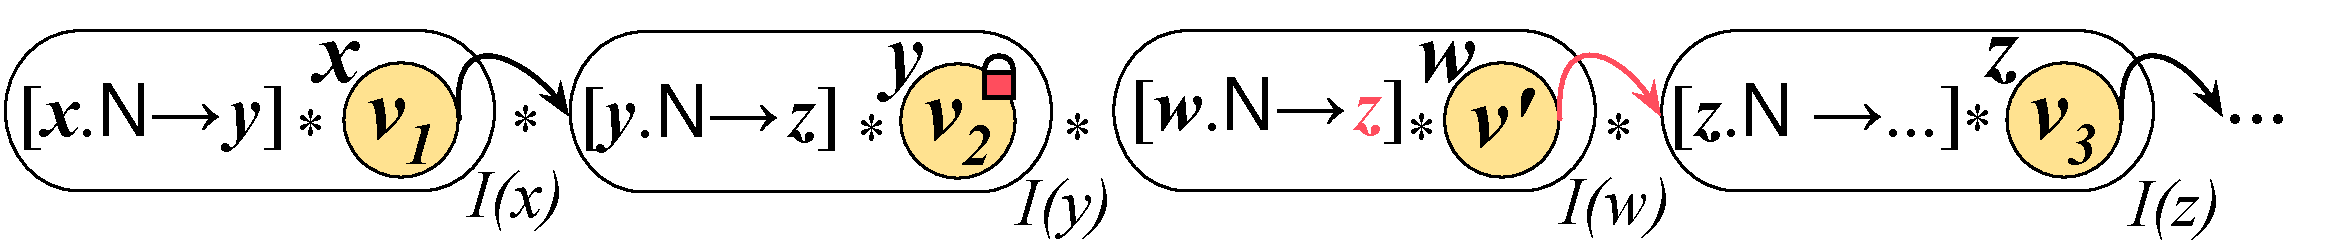
\includegraphics[scale=0.215]{Sections/FurtherExamples/Images/add1.pdf}\\
%
At this point, since the locking thread holds the next pointer of $y$ in its local state, it modifies it to point to the new node $w$. It then unlocks $y$ and returns its next pointer to the shared state. However, the interference assertion associated with node $y$ ($I(y)$) allows the node to be unlocked in three possible ways. Either its successor has not changed from its old value $z$ (tracked by $\nextC{y}{z}$); \emph{or} it has been redirected to $z$'s successor (when $z$ is being deleted); \emph{or} it has been directed to a new node whose successor is $z$ (a new node is inserted between $y$ and $z$). When adding a new node after $y$, the latter of the possibilities is applicable and thus the unlocking thread must demonstrate that the new node ($w$) does indeed point to $z$. In order to establish this condition, we use the (\mergeRule) principle in our reasoning to combine the subjective views of $y$ and $w$ as follows.\\
%
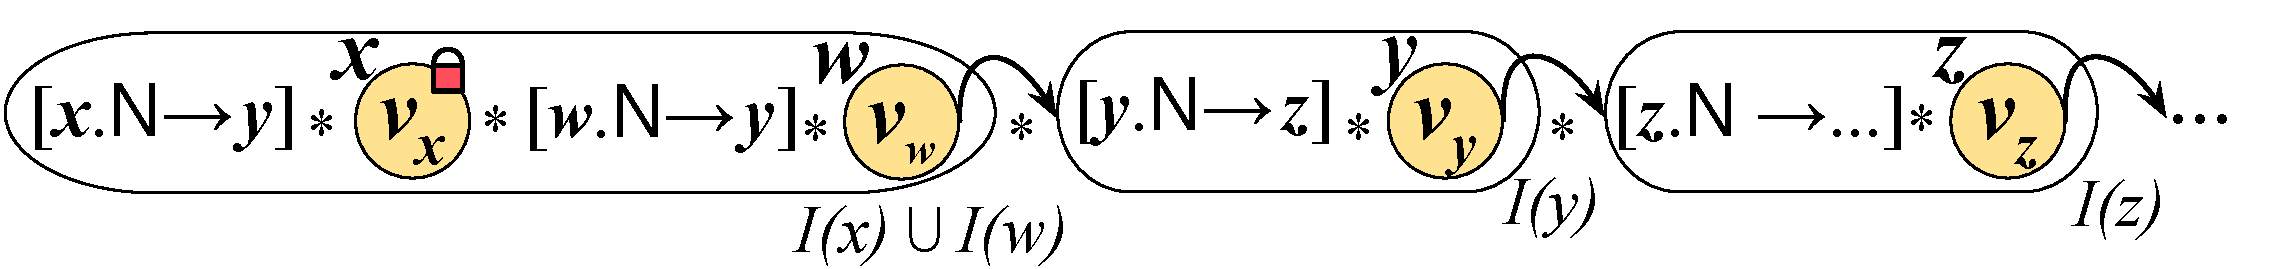
\includegraphics[scale=0.215]{Sections/FurtherExamples/Images/add2.pdf}\\
%
Finally, node $y$ is unlocked; its updated next pointer is returned to the shared state and its next capability is modified accordingly to reflect its new successor. Using the (\copyRule), (\forgetRule) and (\shiftRule) principles \textit{ad seriatim}, we can once again obtain the set predicate with the new node $w$ inserted. \\
%
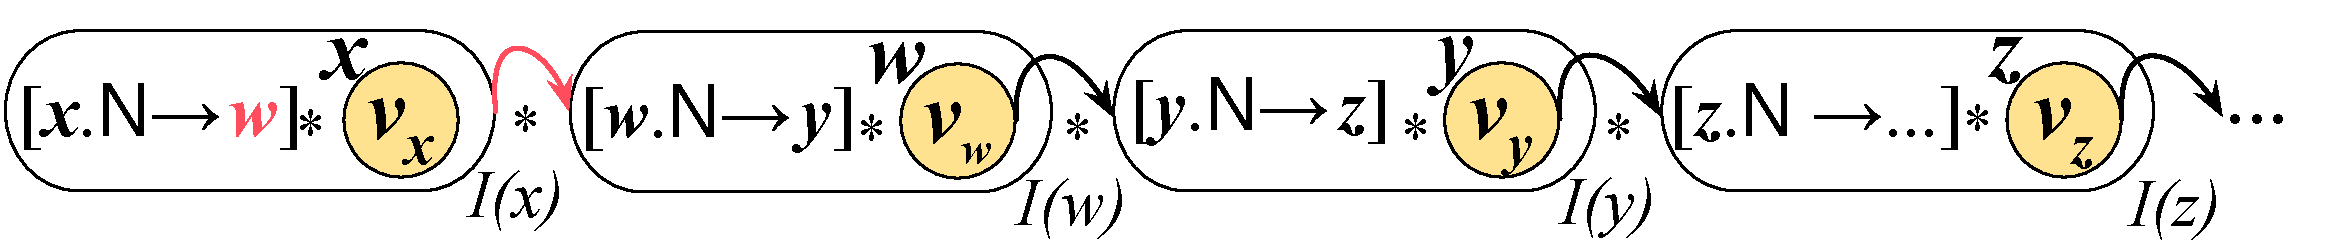
\includegraphics[scale=0.215]{Sections/FurtherExamples/Images/add3.pdf}
%

We can reason about the \li{remove} operation in a similar fashion. Note that the dynamic extension afforded by the \extendRule\ principle allows us to generate new capabilities only when needed and thus gives way to a conciser specification. 
%
Moreover, rather than having a distinct capability to modify the element at address $x$, before address $y$, for each possible successor address $y$ (as with $[\text{U}(x, y, v)]$ in CAP), we appeal to a single capability of the form $\nextC{x}{y}$ whereby the capability is modified accordingly to record the changes to the successor address as demonstrated above. 
%
Lastly, using the reasoning principles of \mergeRule, \forgetRule, \shiftRule\ and \copyRule, we can grow and shrink our subjective views as needed and consequently at any one point we only view the relevant parts of the shared state. 
%
The full \colosl\ specification of the set module as well as the specification proofs are provided in~\cite{colosl-tr14}.
%in that it limits the modifications on node $x$ with respect to its successor $y$. For instance, in order to remove the node at address $y$, a thread proceeds by first acquiring the locks on both $x$ and $y$ nodes. It then claims $x$'s next pointer and redirects it to $z$. In order to ensure that the thread indeed redirects $x$ to $z$ and not any arbitrary address, the we track the current successor of $x$ with $\nextC{x}{y}$ and consequently, in our reasoning, when the thread attempts to unlock $x$, its new successor is compared against the old one $y$ and only when  t of $y$  nodes at $x$ and $y$ when node $x$ is locked and the its next pointer has been temporarily claimed by the locking thread, 


%
%%
%\[
%\begin{array}{@{} r @{\hspace*{3pt}} c @{\hspace*{3pt}} l @{}}
%	\left\{ \inSet{\var{h}}{\var{v}} \right\} & \command{contains(h,v)} & \left\{ \inSet{\var{h}}{\var{v}} * \var{ret} = 1 \right\} \\
%	
%	\left\{ \outSet{\var{h}}{\var{v}} \right\} & \command{contains(h,v)} & \left\{ \outSet{\var{h}}{\var{v}} * \var{ret} = 0 \right\} \\
%	
%	\left\{ \inSet{\var{h}}{\var{v}} \lor \outSet{\var{h}}{\var{v}}  \right\} & \command{add(h,v)} & \left\{ \inSet{\var{h}}{\var{v}} \right\}\\ 
%	
%	\left\{ \inSet{\var{h}}{\var{v}} \lor \outSet{\var{h}}{\var{v}}  \right\} & \command{remove(h,v)} & \left\{ \outSet{\var{h}}{\var{v}} \right\} 
%\end{array}
%\]
%%
%\fig\ref{fig:coloslSetExample} shows a specification of the set module in \colosl\ similar to that of Concurrent Abstract Predicates (CAP) defined in \cite{cap-ecoop10}. We provide the implementation of the set operations as well as the specification proofs in \cite{colosl-tr14}. All three operations proceed by  traversing the sorted list at head address $h$ and locating the first node in the list holding a value $v'$ greater than or equal to $v$. The algorithm for locating such a node begins by locking the head node of the list. It then moves down the list by hand-over-hand locking whereby first the node following the one currently held is locked and then the previously locked node is released. No thread can access a node locked by another thread or traverse past it. As such, no thread can overtake an other thread in accessing the list. 
%We provide a similar specification for the set module in \colosl\ as illustrated in \fig\ref{fig:coloslSetExample}. 
%In what follows we first give a description of the predicates of \fig\ref{fig:coloslSetExample} and subsequently contrast our specification with that of CAP.
%%%
%%\begin{figure*}
%%\hrule
%%\[
%%\begin{array}{@{} l @{}}
%%	\begin{array}{@{} r @{\hspace*{3pt}} l @{}}
%%		\inSet{h}{v} \eqdef & \exsts{\pi} \isLock{h.lock}{\pi} * \valueC{h}{v} * \inList{h}{v}\\
%%	
%%		\outSet{h}{v} \eqdef & \exsts{\pi} \isLock{h.lock}{\pi} * \valueC{h}{v} * \outList{h}{v}\\
%%		
%%		\sortedList{\triangleleft}{h}{v} \eqdef & \exsts{L} \sorted{L} \land v  \triangleleft L \land \lsg{h}{\li{null}}{-\infty:: L ++ \{\infty\} }{h} \hspace{1cm}\text{ where } \triangleleft = \in \text{ or } \triangleleft = \not\in \\
%%	
%%	%	\sorted{L} \eqdef & (L  = [] \land \emp) \lor( \exsts{v_0} L = [v_0] \land \emp) \lor \exsts{v_0, v_1, L'} L = v_0 :: (v_1 :: L') \land v_0 < v_1 \land \sorted{v_1:: L'}\\
%%	
%%		\lsg{x}{y}{L}{h} \eqdef & (L = [] \land x = y \land \emp) \lor (\exsts{z, v, L'} L = v::L' \land \shared{\unlockedNode{x}{v}{z} \lor \lockedNode{x}{v}{z}}{I(h, x)} * \lsg{z}{y}{L'}{h})
%%		
%%	\end{array}\\
%%	
%%	\begin{array}{@{} r l @{\hspace{1.5cm}} r l @{}}
%%		\isLock{a}{\pi} \eqdef & [\lockT{a}[\pi] ] * \shared{\left(\cell{a}{0} * \unlockT{a}\right) \lor \cell{a}{1}}{L(a)}
%%		& \locked{a} \eqdef & [\unlockT{a}] *  \shared{\cell{a}{1}}{L(a)}\\
%%		
%%		\unlockedNode{a}{v}{b} \eqdef & \link{a}{b} * \val{a}{v}{b}
%%		& \lockedNode{a}{v}{b} \eqdef & \locked{a} * \val{a}{v}{b}\\
%%		
%%		\link{a}{b} \eqdef & \cell{a.next}{b} * \isLock{b.lock}{1} * \modC{a}
%%		& \val{a}{v}{b} \eqdef & \cell{a.value}{v} * \nextC{a}{b}
%%	\end{array}\\
%%		
%%%		\node{a}{v}{b} \eqdef & (\link{a}{b} \lor \locked{a}) * \val{a}{v}{b}\\
%%%
%%%		\link{a}{b} \eqdef & \cell{a.next}{b} * \isLock{b}{1} * \modC{a}
%%%		\hspace*{2cm} \val{a}{v}{b} \eqdef  \cell{a.value}{v} * \nextC{a}{b}\\		
%%%		\isLock{a}{\pi} \eqdef & \lockC{a}[\pi] * \shared{\cell{a.lock}{0} * \unlockC{a} \lor \cell{a.lock}{1}}{}
%%%		& \locked{a} \eqdef & \unlockC{a} * \shared{\cell{a.lock}{1}}{}
%%	
%%
%%		
%%%%	I(h, a) \eqdef 
%%%%	\left\{
%%%%	\begin{array}{@{} r @ {\hspace*{2pt}}l @{} }
%%%%%		\text{//Locking}\hspace*{1.4cm}&\\
%%%%		\lockT{a}: &\left\{ \exsts{v, b} \unlockedNode{a}{v}{b} \swap \lockedNode{a}{v}{b}\right\}\\
%%%%		
%%%%%		\text{//Unlocking}\hspace*{1.1cm}&\\
%%%%		\unlockT{a}: & \left\{ \exsts{v, b} \lockedNode{a}{v}{b} \swap \unlockedNode{a}{v}{b}\right\}\\ 
%%%%		
%%%%%		\text{//Deletion of } v \hspace*{0.8cm}&\\
%%%%		\unlockT{a} * \valueT{h}{v}: &
%%%%		\left\{
%%%%		\begin{array}{@{} l @{}}
%%%%			\exsts{v_0, b, c} \lockedNode{a}{v_0}{b} * \lockedNode{b}{v}{c} \swap \lockedNode{a}{v_0}{c} * \lockedNode{b}{v}{c}\\
%%%%			\exsts{v_0, b, c} \lockedNode{b}{v_0}{c} * \lockedNode{a}{v}{c} \swap \lockedNode{b}{v_0}{c}
%%%%			
%%%%		\end{array}
%%%%		\right\}\\ 
%%%%
%%%%		
%%%%%		\text{//Insertion of } v \hspace*{0.7cm}&\\
%%%%		\unlockT{a} * \valueT{h}{v}: &
%%%%		\left\{
%%%%		\begin{array}{@{} l @{}}
%%%%			\exsts{v_1, v_2, c, d} v_1 < v < v_2 \land \lockedNode{a}{v_1}{c} * \lockedNode{c}{v_2}{d} 
%%%%			 \swap \lockedNode{a}{v_1}{b} * \node{b}{v}{c} *  \lockedNode{c}{v_1}{d}\\
%%%%			 
%%%%			 \exsts{v_1, v_2, c, d} v_1 < v < v_2 \land \lockedNode{a}{v_1}{c} * \unlockedNode{c}{v_2}{d} 
%%%%			\swap \lockedNode{a}{v_1}{b} * \node{b}{v}{c} *  \unlockedNode{c}{v_1}{d}
%%%%						
%%%%		\end{array}
%%%%		\right\}\\ 
%%%%		
%%%%	\end{array}
%%%%	\right\}
%%
%%\end{array}
%%\]
%%\hrule
%%\caption{\colosl\ set module specification where the definition of $I(h, v)$ is provided in \cite{colosl-tr14}.}
%%\label{fig:coloslSetExample}
%%\end{figure*}
%%%
%
%%
%\begin{figure*}
%\hrule
%\[
%\begin{array}{r @{} l}
%	\inSet{h}{v} \eqdef &\exsts{\pi} \isLock{h}{\pi} *  \valueC{h}{v} * \inList{h}{v}
%	\hspace{1.5cm}
%	\outSet{h}{v} \eqdef \exsts{\pi} \isLock{h}{\pi} * \valueC{h}{v} * \outList{h}{v}\\
%	
%	\sortedList{\triangleleft}{h}{v} \eqdef & \exsts{L} \sorted{L} \land v  \triangleleft L \land \lsg{h}{\li{null}}{-\infty:: L ++ \{\infty\} }{h} \hspace{1cm}\text{ where } \triangleleft = \in \text{ or } \triangleleft = \not\in \\
%	
%	\lsg{x}{y}{L}{h} \eqdef & (L = [] \land x = y \land \emp) \lor (\exsts{z, v, L'} L = v::L' \land \shared{\node{x}{v}{z}}{I(h, x)} * \lsg{z}{y}{L'}{h})\\
%	
%	\node{a}{v}{b} \eqdef & \unlockedNode{a}{v}{b} \lor \lockedNode{a}{v}{b}
%	\hspace{0.85cm}
%	\unlockedNode{a}{v}{b}  \eqdef \link{a}{b} * \val{a}{v}{b}
%	\hspace{0.85cm}
%	\lockedNode{a}{v}{b} \eqdef  \locked{a} * \val{a}{v}{b}\\
%	
%	\link{a}{b} \eqdef & \cell{a.next}{b} * \isLock{b}{1} * \modC{a}
%	\hspace{4cm}
%	\val{a}{v}{b} \eqdef  \cell{a.value}{v} * \nextC{a}{b}	\\
%	
%	\isLock{a}{\pi} \eqdef & \lockC{a}[\pi] * \shared{\cell{a.lock}{0} * \unlockC{a} \lor \cell{a.lock}{1}}{L(a)}
%	\hspace{1.77cm}
%	\locked{a} \eqdef  \unlockC{a} * \shared{\cell{a.lock}{1}}{L(a)}
%	
%\end{array}
%\]
%%
%\hrule
%\caption{\colosl\ set module specification where the definition of $I(h, v)$ is provided in \cite{colosl-tr14}.}
%\label{fig:coloslSetExample}
%\end{figure*}
%%
%
%Since \colosl is parametric in the separation algebra of capabilities and capability assertions, we instantiate it with a \emph{ghost fractional heap} to represent the separation algebra of capabilities and write heap-like assertions of the form $\setCap{a}[\pi][b]$ to denote capability $a$ with permission $\pi$. Moreover, our capabilities are \emph{stateful} in that they can capture some additional information ($b$). As we demonstrate below, this leads to conciser specifications. For readability we write $\setCap{a}[][b]$ for $\setCap{a}[1][b]$, $\setCap{a}[\pi]$ for $\exsts{b}\setCap{a}[\pi][b]$ and $a$ for $\exsts{b}\setCap{a}[1][b]$.

%\noindent\textbf{\textsf{isLock}($a, \pi$) / \textsf{locked}($a$)} \hspace{0.3cm} 
%Every node in the singly-linked list is protected by a lock that is to be acquired prior to modification of the node. The $\isLock{a}{\pi}$ predicate is similar to that in \cite{cap-ecoop10} and states that the lock at address $a$ can be acquired with permission $\pi \in (0, 1]$. Multiple threads may attempt to acquire the lock at once and thus we use the $\pi$ argument to reflect this sharing where $1$ denotes exclusive right to acquisition while $\pi \in (0, 1)$ accounts for sharing of the lock between multiple threads. The $\isLock{a}{\pi}$ predicate asserts that the thread's local state contains the capability $\lockT{a}[\pi]$ to acquire the lock and that the lock resides in the shared state where at any one point either the lock is unlocked ($\cell{a}{0}$) and the shared state contains the capability to unlock it ($\unlockT{a}$); or it is locked ($\cell{a}{1}$) and the unlocking capability has been claimed by the locking thread. The $\locked{a}$ predicate asserts that the thread's local state contains the exclusive capability to unlock the lock $[\unlockT{a}]$ and that the $a$ is in the locked state ($\cell{a}{1}$). 
%
%\noindent\textbf{\textsf{in}($h, v$) / \textsf{out}($h, v$)} \hspace{0.3cm}
%The $\inSet{h}{v}$ predicate states that the set at head address $h$ contains value $v$ and captures exclusive right to alter the set by changing whether $v$ belongs to it. It asserts that the thread owns some capability ($\pi$) to acquire the lock associated with head address ($\isLock{h}{\pi}$) and that the thread owns the exclusive capability to alter the set with respect to value $v$ ($\valueC{h}{v}$) should it own the capability to modify the address at which value $v$ is stored (\textit{cf.} $\unlockedNode{a}{v}{b}$). The underlying singly-inked list is captured by the $\inList{h}{v}$ predicate. 
%The $\inList{h}{v}$ predicate uses an auxiliary carrier sorted list $L$ (such that $v \in L$) to capture the contents of the singly-linked list via the $\textsf{lsg}$ predicate. For simpler implementation, we extend $L$ with two sentinel values $-\infty$ and $\infty$, one at each end to avoid corner cases such as removing the first/last element of the list. The $\outSet{h}{v}$ predicate is analogous to $\inSet{h}{v}$ and corresponds to the case where the set at address $h$ does not contain $v$.
%
%\noindent\textbf{\textsf{lsg}($x, y, L, h$)} \hspace{0.3cm} This predicate is defined inductively and describes a \emph{segment} of the list at $h$ that starts at address $x$ and extends upto (but not including) address $y$ and contains the elements in the mathematical list $L$. When $L$ is empty, it corresponds to a void segment and yields no resources (\emp); otherwise, it is defined as the composition of the first node of the segment at address $x$, $\shared{\node{x}{v}{z}}{I(h, x)}$, and the tail of the list segment ($\lsg{z}{y}{L'}{h}$). The $\node{x}{v}{z}$ predicate describes a node at address $x$ with value $v$ and successor $z$ and can be either unlocked ($\unlockedNode{x}{v}{z}$) or locked ($\lockedNode{x}{v}{z}$).
%
%\noindent\textbf{\textsf{U}($a, v, b$) / \textsf{L}($a, v, b$)} \hspace{0.3cm}
%%The $\unlockedNode{a}{v}{b}$ predicate states that the node at address $a$ is unlocked, it contains value $v$ and comes before the node at address $b$. The statement of the $\lockedNode{a}{v}{b}$ predicate is analogous and describes the node when locked.
%%In both locked and unlocked states, the shared state contains the lock field ($\cell{a}{0}$ or $\cell{a}{1}$), the value field ($\cell{a+1}{v}$) and the capability that records the current successor of the node $\nextC{a}{b}$.
%%When a node is in the unlocked state, the shared state contains the next pointer of the node ($\cell{a+2}{b}$), as well as the capability to unlock the node ($[\unlockT{a}]$).
%%% A thread can alter the set at $h$ with respect to the node at $a$ with value $v$ only when it holds both the value capability $\valueC{h}{v}$ and the modification capability $\modC{a}$ in its local state. 
%%Recall that when traversing the list by hand-over-hand locking, no thread can overtake an other in traversing the list. Consequently, a node can only be locked by a thread that has already acquired the lock associated with the previous node. 
%%As such, when the node $a$ is in the unlocked state, the exclusive capability to lock the successor node at address $b$ ($[\lockT{b}]$) also lies in the shared state.
%%% 
%%
%%When a thread successfully locks the node at $a$ it claims the next pointer, the unlocking capability and the locking capability pertaining to its successors. ($\cell{a.next}{b} * [\unlockT{a}] * [\lockT{b}]$) and moves them into its local state.
%%\\
%%
%A thread can alter the set at $h$ with respect to the node at address $a$ with value $v$, only when it holds both the value capability $\valueC{h}{v}$ and the modification capability $\modC{a}$ in its local state. When the node is in the unlocked state, no thread can modify it and thus the modification capability $\modC{a}$ as well as the next pointer of the node ($\cell{a.next}{b}$) lie in the shared state. 
%%
%Recall that when traversing the list by hand-over-hand locking, no thread can overtake an other in traversing the list. Consequently, a node can only be locked by a thread that has already acquired the lock associated with the previous node. Therefore, when the node $a$ is in the unlocked state, the exclusive capability to lock its successor at address $b$ ($\isLock{b}{1}$) also lies in the shared state.
%%
%When a thread successfully locks the node at $a$, it claims the next pointer, the modification capability and the locking capability pertaining to its successors ($\link{a}{b}$), and moves them into its local state. In return, it transfers the $\locked{a}$ resource to the shared state as evidence that it is indeed the thread that has acquired the lock. 
%
%In both locked and unlocked states, the shared state contains the value field ($\cell{a.value}{v}$) and the ``successor'' capability $\nextC{a}{b}$. This capability is used to track the current successor of $a$ even when the node is locked and its next pointer has been claimed by the locking thread. 
%% 
%\\

%%Note that for simplicity, rather than using a separate lock module in our set specification as in the case of \cite{cap-ecoop10}, we extend the representation of each node to contain a simple compare-and-swap lock. 
%The definitions of most of the predicates in \fig\ref{fig:coloslSetExample} are analogous to the correspondingly-named predicates in \cite{cap-ecoop10} specified in CAP. The difference however lies in the definitions of the 
%$\textsf{L}_{\triangleleft}$ and \textsf{lsg} predicates. 
%\fig\ref{fig:capSetExample} presents the definitions of these predicates in CAP as specified in \cite{cap-ecoop10}. 
%There are two main advantages to the \colosl\ specification of the set module. In the CAP specification all elements of the set (represented as a singly-linked list) reside in a shared region labelled $s$. Since the capabilities associated with a region are all allocated at the point of region creation, the shared region is required to keep track of all possible update capabilities $\capGapT{a}{b}{v}$ associated with all addresses $a$, all possible successor addresses $b$ and all values $v$. For instance, since the value $v$ may be contained in the set at address $x$ before address $y$, the region must include the $\capGapT{a}{b}{v}$ capability to accommodate possible modifications of value $v$. This is captured by the $\gapsCAP{S}{s}$ and $\myGapsCAP{S}{s}$ predicates through the infinite multiplicative star operator $\iterStar$. The $\gapsCAP{S}{s}$ predicate uses an auxiliary mathematical set $S$ to track those nodes of the list that are currently locked and thus infer which \textsc{LGap} capabilities reside in the shared state and which ones have been removed. This results in an inevitably cluttered and a rather counter-intuitive specification since it seems unnatural to account for the capabilities pertaining to addresses not in the domain of the set. On the other hand, in the \colosl\ specification we use a combination of the $\modT{a}$ and $\nextT{a}{b}$ capabilities to achieve the same effect for each address $a$. Since \colosl\ allows for dynamic extension of the shared state, the capabilities associated with each address ($a$) are generated upon extension of the shared state with those addresses, and therefore it is not necessary to account for capabilities concerning those addresses absent from the list. 
%
%Moreover, since the ghost heaps used to represent the separation algebra of capabilities are \emph{stateful}, rather than having a distinct capability to modify the element at address $a$ before address $b$ for each possible successor address $b$, we appeal to a single capability of the form $\nextT{a}{b}$ whereby the capability is modified accordingly to reflect the changes to the successor address. For instance, when node at address $a$ is redirected to point from address $b$ to a new location at address $c$, $\nextT{a}{b}$ is also updated as $\nextT{a}{c}$. 

%%
%\begin{figure*}
%\hrule
%\[
%\begin{array}{@{} l @{}}
%	\begin{array}{@{} r @{\hspace*{3pt}} l @{}}
%	
%		\sortedListCAP{\triangleleft}{h}{v}{s} \eqdef & \exsts{L, S} \sorted{L} \land v  \triangleleft L \land \lsgCAP{h}{\li{null}}{S}{-\infty:: L ++ \{\infty\} } * \shade{\left( \gapsCAP{S}{s} \land \myGapsCAP{v}{s} \right) } \text{ where } \triangleleft = \in \text{ or } \triangleleft = \not\in \\
%	  
%	
%		\lsg{x}{y}{S}{L} \eqdef & (L = [] \land S = \emptyset \land x = y \land \emp) \lor (\exsts{z, v, L'} L = v::L' \land \unlockedNode{x}{v}{z} * \lsg{z}{y}{S}{L'})\\
%		
%		& \lor (\exsts{z, v, L', S'} L = v::L' \land S = \{(x, z)\} \uplus S' \land \lockedNode{x}{v}{z} * \lsg{z}{y}{S'}{L'})
%		
%	\end{array}\\
%	
%		
%		
%	\shade{
%	\begin{array}{@{} r @{\hspace*{3pt}} l @{}}
%		\gapsCAP{S}{s} \eqdef & \iterStar(x, y) \not\in S. \iterStar v. \capGapC{x}{y}{v}{s} *\\
%		& \iterStar (x, y) \in S. \exsts{w} \iterStar v \not= w. \capGapC{x}{y}{v}{s} \land \\
%		&\for{x, y, w, z} (x, y) \in S \land (w, z) \in S \implies (x = w \iff y = z) \\
%		
%	  \myGapsCAP{v}{s} \eqdef & \iterStar x, y. \capGapC{x}{y}{v}{s} * true \\
%		
%	\end{array}
%	}
%\end{array}
%\]
%\hrule
%\caption{CAP predicates of the set module that contrast with the \colosl\ specification of \fig\ref{fig:coloslSetExample}.}
%\label{fig:capSetExample}
%\end{figure*}
